% Options for packages loaded elsewhere
\PassOptionsToPackage{unicode,linktoc=all}{hyperref}
\PassOptionsToPackage{hyphens}{url}
\PassOptionsToPackage{dvipsnames,svgnames,x11names}{xcolor}
%
\documentclass[
  a4paper,
]{article}
\usepackage{amsmath,amssymb}
\usepackage{lmodern}
\usepackage{iftex}
\ifPDFTeX
  \usepackage[T1]{fontenc}
  \usepackage[utf8]{inputenc}
  \usepackage{textcomp} % provide euro and other symbols
\else % if luatex or xetex
  \usepackage{unicode-math}
  \defaultfontfeatures{Scale=MatchLowercase}
  \defaultfontfeatures[\rmfamily]{Ligatures=TeX,Scale=1}
\fi
% Use upquote if available, for straight quotes in verbatim environments
\IfFileExists{upquote.sty}{\usepackage{upquote}}{}
\IfFileExists{microtype.sty}{% use microtype if available
  \usepackage[]{microtype}
  \UseMicrotypeSet[protrusion]{basicmath} % disable protrusion for tt fonts
}{}
\makeatletter
\@ifundefined{KOMAClassName}{% if non-KOMA class
  \IfFileExists{parskip.sty}{%
    \usepackage{parskip}
  }{% else
    \setlength{\parindent}{0pt}
    \setlength{\parskip}{6pt plus 2pt minus 1pt}}
}{% if KOMA class
  \KOMAoptions{parskip=half}}
\makeatother
\usepackage{xcolor}
\IfFileExists{xurl.sty}{\usepackage{xurl}}{} % add URL line breaks if available
\IfFileExists{bookmark.sty}{\usepackage{bookmark}}{\usepackage{hyperref}}
\hypersetup{
  pdftitle={Reflections on the Mind of Nikola Tesla},
  pdfauthor={R (Chandra) Chandrasekhar},
  pdflang={en-GB},
  colorlinks=true,
  linkcolor={DarkOliveGreen},
  filecolor={Purple},
  citecolor={DarkKhaki},
  urlcolor={Maroon},
  pdfcreator={LaTeX via pandoc}}
\urlstyle{same} % disable monospaced font for URLs
\usepackage[margin=25mm]{geometry}
\usepackage{graphicx}
\makeatletter
\def\maxwidth{\ifdim\Gin@nat@width>\linewidth\linewidth\else\Gin@nat@width\fi}
\def\maxheight{\ifdim\Gin@nat@height>\textheight\textheight\else\Gin@nat@height\fi}
\makeatother
% Scale images if necessary, so that they will not overflow the page
% margins by default, and it is still possible to overwrite the defaults
% using explicit options in \includegraphics[width, height, ...]{}
\setkeys{Gin}{width=\maxwidth,height=\maxheight,keepaspectratio}
% Set default figure placement to htbp
\makeatletter
\def\fps@figure{htbp}
\makeatother
\setlength{\emergencystretch}{3em} % prevent overfull lines
\providecommand{\tightlist}{%
  \setlength{\itemsep}{0pt}\setlength{\parskip}{0pt}}
\setcounter{secnumdepth}{-\maxdimen} % remove section numbering
\newlength{\cslhangindent}
\setlength{\cslhangindent}{1.5em}
\newlength{\csllabelwidth}
\setlength{\csllabelwidth}{3em}
\newlength{\cslentryspacingunit} % times entry-spacing
\setlength{\cslentryspacingunit}{\parskip}
\newenvironment{CSLReferences}[2] % #1 hanging-ident, #2 entry spacing
 {% don't indent paragraphs
  \setlength{\parindent}{0pt}
  % turn on hanging indent if param 1 is 1
  \ifodd #1
  \let\oldpar\par
  \def\par{\hangindent=\cslhangindent\oldpar}
  \fi
  % set entry spacing
  \setlength{\parskip}{#2\cslentryspacingunit}
 }%
 {}
\usepackage{calc}
\newcommand{\CSLBlock}[1]{#1\hfill\break}
\newcommand{\CSLLeftMargin}[1]{\parbox[t]{\csllabelwidth}{#1}}
\newcommand{\CSLRightInline}[1]{\parbox[t]{\linewidth - \csllabelwidth}{#1}\break}
\newcommand{\CSLIndent}[1]{\hspace{\cslhangindent}#1}
\ifLuaTeX
\usepackage[bidi=basic]{babel}
\else
\usepackage[bidi=default]{babel}
\fi
\babelprovide[main,import]{british}
% get rid of language-specific shorthands (see #6817):
\let\LanguageShortHands\languageshorthands
\def\languageshorthands#1{}
% $HOME/.pandoc/defaults/latex-header-includes.tex
% Common header includes for both lualatex and xelatex engines.
%
% Preliminaries
%
\PassOptionsToPackage{rgb,dvipsnames,svgnames}{xcolor}
\PassOptionsToPackage{main=british}{babel}
\AtBeginEnvironment{quote}{\small}
\AtBeginEnvironment{quotation}{\small}
\AtBeginEnvironment{longtable}{\centering}
%
% Packages that are useful to include
%
\usepackage{graphicx}
\usepackage{subcaption}
\usepackage[inkscapeversion=1]{svg}
\usepackage[defaultlines=4,all]{nowidow}
\usepackage[capitalize,noabbrev]{cleveref}
\usepackage{etoolbox}
\usepackage{fontsize}
\usepackage{newunicodechar}
\usepackage{pdflscape}
\usepackage{fnpct}
\usepackage{parskip}
  \setlength{\parindent}{0pt}
\usepackage[style=american]{csquotes}
% \usepackage{setspace} Use the <fontname-plus.tex> files for setspace
%
% charis-plus.tex
% Font-setting header file for use with Pandoc Markdown
% to generate PDF via LuaLaTeX.
% The main font is Charis SIL.
% Other main fonts are also available in appropriately named file.
\usepackage{fontspec}
\usepackage{setspace}
\setstretch{1.3}
%
\defaultfontfeatures{Ligatures=TeX,Scale=MatchLowercase,Renderer=HarfBuzz} % at the start always
%
% For English
%
\babelfont{rm}[Scale=1]{Merriweather}
\babelfont{sf}[BoldFont={* Semibold}]{Source Sans Pro}
\babelfont{tt}[Scale=0.9]{Fira Mono}
%
\babelprovide[import,onchar=ids fonts]{sanskrit}
\babelprovide[import,onchar=ids fonts]{tamil}
\babelprovide[import,onchar=ids fonts]{greek}
%
\babelfont[sanskrit]{rm}[Scale=1.1,Renderer=HarfBuzz]{Noto Serif Devanagari}
\babelfont[sanskrit]{sf}[Scale=1.1,Renderer=HarfBuzz]{Noto Sans Devanagari}
\babelfont[tamil]{rm}[Renderer=HarfBuzz]{Noto Serif Tamil}
\babelfont[tamil]{sf}[Renderer=HarfBuzz]{Noto Sans Tamil}
\babelfont[greek]{rm}{Gentium Book Plus}
%
% Math font
%
\usepackage{unicode-math} % seems not to hurt % fallabck
\setmathfont[bold-style=TeX]{STIX Two Math}
%
% Other fonts
%
\newfontfamily{\emojifont}{Symbola}
%
\usepackage{titling}
\usepackage{fancyhdr}
    \pagestyle{fancy}
    \fancyhead{}
    \fancyfoot{}
    \renewcommand{\headrulewidth}{0.2pt}
    \renewcommand{\footrulewidth}{0.2pt}
    \fancyhead[LO,RE]{\scshape\thetitle}
    \fancyfoot[CO,CE]{\footnotesize Copyright © 2006\textendash\the\year, R (Chandra) Chandrasekhar}
    \fancyfoot[RE,RO]{\thepage}
\newfontfamily{\regulariconfont}{Font Awesome 6 Free Regular}[Color=Grey]
\newfontfamily{\solidiconfont}{Font Awesome 6 Free Solid}[Color=Grey]
\newfontfamily{\brandsiconfont}{Font Awesome 6 Brands}[Color=Grey]
%
% Direct input of Unicode code points
%
\newcommand{\faEnvelope}{\regulariconfont\ ^^^^f0e0\normalfont}
\newcommand{\faMobile}{\solidiconfont\ ^^^^f3cd\normalfont}
\newcommand{\faLinkedin}{\brandsiconfont\ ^^^^f0e1\normalfont}
\newcommand{\faGithub}{\brandsiconfont\ ^^^^f09b\normalfont}
\newcommand{\faAtom}{\solidiconfont\ ^^^^f5d2\normalfont}
\newcommand{\faPaperPlaneRegular}{\regulariconfont\ ^^^^f1d8\normalfont}
\newcommand{\faPaperPlaneSolid}{\solidiconfont\ ^^^^f1d8\normalfont}

%
% The block below is commented out because of Tofu glyphs in HTML
%
% \newcommand{\faEnvelope}{\regulariconfont\ \normalfont}
% \newcommand{\faMobile}{\solidiconfont\ \normalfont}
% \newcommand{\faLinkedin}{\brandsiconfont\ \normalfont}
% \newcommand{\faGithub}{\brandsiconfont\ \normalfont}
\ifLuaTeX
  \usepackage{selnolig}  % disable illegal ligatures
\fi

\title{Reflections on the Mind of Nikola Tesla}
\author{R (Chandra) Chandrasekhar}
\date{2006-06-05 | 2021-02-18}

\begin{document}
\maketitle




\begin{quote}
This ``blog'' was originally an academic paper that was submitted for
publication in the prestigious journal
\href{https://proceedingsoftheieee.ieee.org/}{\emph{Proceedings of the
IEEE}} in 2006, the year of Tesla's 150th birth anniversary. Although
well-received by some, it was, alas, rejected. That same manuscript has
been augmented, updated, and reformatted here, to be shared with the
wider world. Hyperlinks have been added for the convenience of the
reader. I apologize if this blog reads like a \emph{slog}.
\emojifont{😉}\normalfont
\end{quote}

\hypertarget{introduction}{%
\subsection{Introduction}\label{introduction}}

Nikola Tesla was a prodigious genius who benefited mankind immensely. He
embodied a strange combination of fiery imagination, more suited to the
poet or artist, tempered by the discipline of the engineer, grounded in
mathematics and experimental science. The fact that he worked mostly
alone and produced baffling inventions has led to his being labelled as
both sorcerer and genius. He was superhuman in his will power and in his
appetite for work. Yet he was also a frail human being who suffered a
nervous breakdown, who had a fixation on the number three, and who, in
later life, made bizarre claims which alienated him from mainstream
science. Although he was well recognized by his scientific peers and the
media in the late nineteenth and early twentieth century, Tesla today
remains a largely unknown and unsung hero, who has not been accorded his
rightful place in history.\footnote{This was written \emph{before} the
  \href{https://en.wikipedia.org/wiki/Tesla,_Inc.}{electric vehicle
  brand Tesla} gained global prominence.} It is also ironic that,
although others profited immensely from his inventions, Tesla himself
did not enjoy a prosperity commensurate with his abilities or
contributions, and died alone and in penury.

\begin{figure}
\hypertarget{fig:tesla}{%
\centering
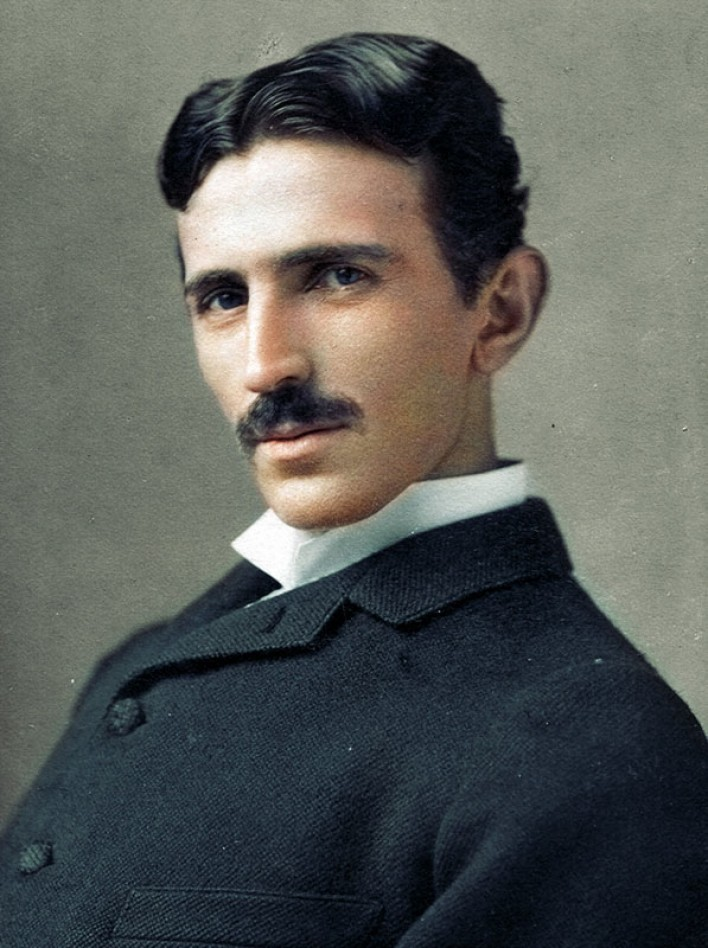
\includegraphics[width=0.8\textwidth,height=\textheight]{images/tesla_in_color.jpg}
\caption[Nikola Tesla at age 34; photograph by
\href{https://en.wikipedia.org/wiki/Napoleon_Sarony}{Napoleon Sarony};
colorized by \href{http://www.danarkeller.com/}{Dana Keller}.]{Nikola
Tesla at age 34; photograph by
\href{https://en.wikipedia.org/wiki/Napoleon_Sarony}{Napoleon Sarony};
colorized by \href{http://www.danarkeller.com/}{Dana
Keller}.\footnotemark{}}\label{fig:tesla}
}
\end{figure}
\footnotetext{The uncoloured image is
  \href{https://commons.wikimedia.org/wiki/File:Tesla_circa_1890.jpeg}{available
  at Wikipedia} and is in the public domain in the US and certain other
  countries.}

It is impossible to review the visionary contributions of Tesla within
the compass of one paper, let alone do justice to analyzing his unique
mind. Only certain aspects of Tesla's mind will concern us here; the
interested reader is referred to brief synopses and fuller accounts of
his life and writings elsewhere
\protect\hyperlink{ref-john83}{{[}1{]}}--\protect\hyperlink{ref-tesla-pbs-bio}{{[}8{]}}.
In this paper, we focus on only four of his documented mental
characteristics:

\begin{enumerate}
\tightlist
\item
  An extremely acute sense of hearing and sight;
\item
  A power of visualization so vivid as to mimic reality;
\item
  Eccentricities of habit and behaviour; and
\item
  Making grandiose claims, some of which remain open until today.
\end{enumerate}

In each case, evidence is furnished from Tesla's own writings, his
biographies, or from the other available literature. Each of these
traits is examined in some detail, especially with respect to his
creativity. Comparisons are made with other well known scientists with
similar characteristics, and speculative comments are made, along with a
list of questions worthy of further investigation. Finally, a hypothesis
is put forward---based on the idea of mental evolution, as proposed by R
M Bucke \protect\hyperlink{ref-bucke48}{{[}9{]}}---as one possible
explanation for Tesla's prodigious and rare mind.

\hypertarget{teslas-hypersensitive-hearing-and-sight}{%
\subsection{Tesla's hypersensitive hearing and
sight}\label{teslas-hypersensitive-hearing-and-sight}}

From a young age, Tesla had hypersensitive hearing and sight. For
example, he recounted \protect\hyperlink{ref-cheney81}{{[}3{]}} that in
his boyhood, he saved his neighbours' lives when he heard the crackling
of flames consuming their homes at night. At the age of 25, he suffered
what was termed by his doctors a ``nervous breakdown'' for want of a
better term. While he was ill, Tesla's pulse varied from a few beats to
two hundred and sixty beats per minute and all the tissues of his body
quivered and twitched \protect\hyperlink{ref-john83}{{[}1{]}}. During
the period he was ill, Tesla had the following extraordinary aural
experiences\protect\hyperlink{ref-john83}{{[}1{]}},
\protect\hyperlink{ref-cheney81}{{[}3{]}}:

\begin{enumerate}
\item
  He could hear the sound of a watch ticking three rooms away;
\item
  A fly landing on a table in his room caused a dull thud in his ear;
\item
  A carriage passing several kilometres distant caused his whole body to
  shake;
\item
  He could not endure the vibration in his chair caused by a train
  whistle thirty-two kilometres away;
\item
  Rubber cushions had to be placed under his bed so that he could rest
  undisturbed by the vibrations of sounds around him; and
\item
  In the dark, like a bat, he could sense an object at a distance of
  about four metres by a peculiar creepy sensation on the forehead.
\end{enumerate}

Even when Tesla was past forty, and conducting research into lightning
in the Colorado mountains, in the USA, he could hear thunderclaps 880
kilometres away, whereas his assistants, at half his age, could only
hear them up to 240 kilometres away
\protect\hyperlink{ref-john83}{{[}1{]}},
\protect\hyperlink{ref-cheney81}{{[}3{]}}.

Not only was his hearing acute, Tesla's sense of sight was incredible.
It enabled him to perform what may be termed \emph{peregrinations of the
mind}. Let us hear it in his own words:

\begin{quote}
In my boyhood I suffered from a peculiar affliction due to the
appearance of images, often accompanied by strong flashes of light,
which marred the sight of real objects and interfered with my thought
and action. They were pictures of things and scenes which I had really
seen, \emph{never of those I imagined}. When a word was spoken to me the
image of the object it designated would present itself vividly to my
vision and sometimes I was quite unable to distinguish whether what I
saw was tangible or not. This caused me great discomfort and
anxiety\ldots{}

Then I instinctively commenced to make excursions beyond the limits of
the small world of which I had knowledge, and I saw new scenes. These
were at first very blurred and indistinct, and would flit away when I
tried to concentrate my attention upon them, but by and by I succeeded
in fixing them; they gained in strength and distinctness and
\emph{finally assumed the concreteness of real things}. I soon
discovered that my best comfort was attained if I simply went on in my
vision farther and farther, getting new impressions all the time, and so
I began to travel---of course, in my mind. Every night (and sometimes
during the day), when alone, I would start on my journeys---see new
places, cities and countries---live there, meet people and make
friendships and acquaintances and, however unbelievable, it is a fact
that they were just as clear to me as those in actual life and not a bit
less intense in their manifestations.
\protect\hyperlink{ref-john83}{{[}1{]}} (\emph{emphasis} is mine)
\end{quote}

Here we see that it was not a hypersensitivity to an actual stimulus,
but the sensation of vision that had verisimilitude, without the need
for any external stimulus, which is singular.

\hypertarget{questions-and-conjectures-hearing-and-sight}{%
\subsubsection{Questions and conjectures: hearing and
sight}\label{questions-and-conjectures-hearing-and-sight}}

The following questions and conjectures arise regarding Tesla's unusual
hearing and sight:

\begin{enumerate}
\tightlist
\item
  Was Tesla's mind influenced in any way by his heightened and unusual
  sensory awareness?
\item
  If so, what was the cause-effect relationship?

  \begin{enumerate}
  \def\labelenumii{\alph{enumii}.}
  \tightlist
  \item
    Were his hyper-acute senses responsible for his mental powers?
  \item
    Or did his sensory acuity arise from his amazing mental faculties?
  \end{enumerate}
\item
  Were his sightseeing journeys a form of vivid daydreaming, or were
  they hallucinations, or were they some other as yet unlabelled
  phenomenon?
\item
  Did his ``nervous breakdown'' influence his inventive abilities?
\item
  Were his eccentric habits and behaviour in later life the sequelae of
  his ``nervous breakdown''?
\end{enumerate}

It is believed that these and other questions posed here are worthy of
further investigation by specialist researchers; the answers to them are
likely to shed light on many aspects of the creative scientific process.

\hypertarget{teslas-vivid-visualization-and-mental-experiments}{%
\subsection{Tesla's vivid visualization and mental
experiments}\label{teslas-vivid-visualization-and-mental-experiments}}

If Tesla's hyper-acute senses marked him out as unusual, his vivid
visualization and extremely efficient method for realizing his
inventions are unique in the annals of the history of science. Tesla not
only discovered hidden forces and sources of energy, but he also
designed machines that made practical use of his discoveries for the
benefit of humanity. Thus, not only was he an applied mathematician and
experimental scientist, he was also a highly accomplished engineer, but
one whose methods were atypical. We will first examine in some detail
the genesis of the invention of the induction motor that came about from
his grasping the idea of rotating magnetic fields. This is followed by a
brief recountal and analysis of the discovery of the benzene ring by the
chemist Friedrich August Kekulé. Then we will explore and discuss
Telsa's vivid faculty of visualization, and compare it with similar
instances from other well known scientists. We conclude this section
with a discussion of the process of scientific discovery and creativity.

\hypertarget{the-ac-induction-motor}{%
\subsubsection{The AC induction motor}\label{the-ac-induction-motor}}

In 1875, at the age of 19, Tesla enrolled at the Polytechnic Institute
at Graz in Austria to study electrical engineering. In his second year
there, his professor demonstrated a direct current (DC) motor for the
first time. Tesla was impressed but objected to the sparking that he saw
taking place at the commutator. His professor replied that the sparking
was inevitable, being inherent in the design of the machine. Tesla was
unconvinced and felt that there must be some way to circumvent the use
of commutators. He felt inwardly assured that there was a solution to
this problem, although his instructors did not share this view
\protect\hyperlink{ref-oneill80}{{[}2{]}}. He later used these words to
describe this inner certitude:

\begin{quote}
In attacking the problem again I almost regretted that the struggle was
soon to end. I had so much energy to spare. When I undertook the task it
was not with a resolve such as men often make. With me it was a sacred
vow, a question of life and death. I knew that I would perish if I
failed. Now I felt that the battle was won. Back in the deep recesses of
the brain was the solution, but I could not yet give it outward
expression. \protect\hyperlink{ref-john83}{{[}1{]}}
\end{quote}

Paradoxically, the demonstration of the DC motor had convinced him that
by using alternating current (AC) with its changing direction of current
flow, the commutator could be eliminated altogether. While he felt an
inner assurance that it could be done, what he did not know was how to
accomplish it \protect\hyperlink{ref-oneill80}{{[}2{]}}. The answer came
to him, not by logical reasoning, but by a flash of insight that he
later described in these words:

\begin{quote}
I could not demonstrate my belief at that time, but it came to me
through what I might call instinct, for lack of a better name. But
instinct is something which transcends knowledge. We undoubtedly have in
our brains some finer fibres which enable us to perceive truths which we
could not attain through logical deduction, and which it would be futile
to attempt to achieve through any wilful effort of thinking.
\protect\hyperlink{ref-oneill80}{{[}2{]}} (p 49).
\end{quote}

After six years of intensive thought, Tesla did finally get the
revelation that revolutionized our world: the AC induction motor and,
concomitantly, the AC generator. It occurred in Budapest during a walk
in the late afternoon that he took with a friend in February 1882. The
full flavour of the revelation that dawned on him is best conveyed by
his own words:

\begin{quote}
One afternoon, which is ever present in my recollection, I was enjoying
a walk with my friend in the City Park and reciting poetry. At that age
I knew entire books by heart, word for word. One of these was Goethe's
\emph{Faust}. The sun was just setting and reminded me of the glorious
passage:

Sie rückt und weicht, der Tag ist überlebt,\\
Dort eilt sie hin und fördert neues Leben.\\
O, daß kein Flügel mich vom Boden hebt,\\
Ihr nach und immer nach zu streben!\\
\ldots{}\\
Ein schöner Traum, indessen sie entweicht,\\
Ach, zu des Geistes Flügeln wird so leicht\\
Kein körperlicher Flügel sich gesellen!\\
\strut \\
The glow retreats, done is the day of toil;\\
It yonder hastes, new fields of life exploring;\\
Ah, that no wing can lift me from the soil\\
Upon its track to follow, follow soaring!\\
\ldots{}\\
A glorious dream! though now the glories fade.\\
Alas! the wings that lift the mind no aid\\
Of wings to lift the body can bequeath me.\\
\strut \\

As I uttered these inspiring words the idea came like a flash of
lightning and in an instant the truth was revealed. I drew with a stick
on the sand the diagrams shown six years later in my address before the
American Institute of Electrical Engineers, and my companion understood
them perfectly. The images I saw were wonderfully sharp and clear and
had the solidity of metal and stone, so much so that I told him: ``See
my motor here; watch me reverse it.'' I cannot begin to describe my
emotions. Pygmalion seeing his statue come to life could not have been
more deeply moved. A thousand secrets of nature which I might have
stumbled upon accidentally I would have given for that one which I had
wrested from her against all odds and at the peril of my existence.
\protect\hyperlink{ref-john83}{{[}1{]}}
\end{quote}

Writing in the \emph{Scientific American}, Tesla explains this
revelation further:

\begin{quote}
It is extremely difficult for me to put this experience before the
reader in its true light and significance for it is so altogether
extraordinary. When an idea presents itself it is, as a rule, crude and
imperfect. Birth, growth and development are phases normal and natural.
It was different with my invention. In the very moment I became
conscious of it, I saw it fully developed and perfected.
\protect\hyperlink{ref-tesla-personal}{{[}10{]}}
\end{quote}

\begin{figure}
\hypertarget{fig:ac-motor}{%
\centering
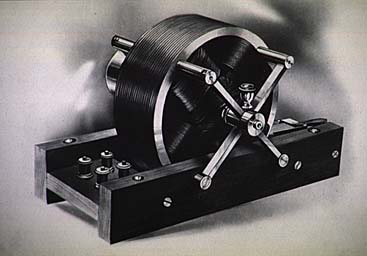
\includegraphics[width=0.8\textwidth,height=\textheight]{images/acmot_main02.jpg}
\caption[The AC induction motor.]{The AC induction
motor.\footnotemark{}}\label{fig:ac-motor}
}
\end{figure}
\footnotetext{This is one of the two two-phase induction motors
  demonstrated by Tesla in his historic lecture of 16 May 1888, before
  the American Institute of Electrical Engineers at Columbia University.
  The motor developed one-half horsepower and showed that brushes and
  commutators could be eliminated. This image and the information in
  this footnote are taken from \href{https://www.pbs.org/tesla/}{the PBS
  (Public Broadcasting System) web site on Tesla}
  \protect\hyperlink{ref-tesla-pbs-bio}{{[}8{]}}.}

In his own mind, the idea of the rotating magnetic fields, one chasing
the other, that formed the basis of the induction motor and the AC
generator, was the greatest secret that he had plucked from Nature. Ever
since he first saw the DC motor with its commutator and sparking, he had
resolved to invent a motor that did away with those features. After six
years of protracted thought and indefatigable effort, he had at last
succeeded, but he paid a price by suffering from a ``nervous breakdown''
soon thereafter.

\hypertarget{archimedes-the-eureka-moment-and-incubation}{%
\subsubsection{Archimedes, the eureka moment, and
incubation}\label{archimedes-the-eureka-moment-and-incubation}}

There are two well-known instances of scientific discoveries that
occurred as flashes of insight after protracted mental effort at problem
solving, not unlike Tesla's vision of the rotating magnetic fields. The
first is that of
\href{https://en.wikipedia.org/wiki/Archimedes}{Archimedes of Syracuse}
as he was in his bath. When he saw the water overflow as he sank into
the bath, he spontaneously saw
\href{https://en.wikipedia.org/wiki/Archimedes\#Archimedes'_principle}{the
solution to his problem}. Oblivious to his nakedness, he ran unclad
along the streets of Syracuse, proclaiming ``Eureka!'' (I have found
it!). Such nodal points of scientific discovery may be called
\emph{eureka moments}.

Tesla's eureka moment regarding the induction motor, and conversely AC
power generation, occurred during an evening walk with his friend, as we
have already seen. Such insights are often the result of sustained
thinking on a topic, with a subsequent relaxation, as in Archimedes's
bath or Tesla's walk, when unheralded, ``the penny drops'' and the
solution is revealed, apparently without any immediate conscious effort
on the part of the scientist. The mathematician
\href{https://en.wikipedia.org/wiki/Henri_Poincar\%C3\%A9}{Jules Henri
Poincaré} believed that after prolonged thinking on a problem, there is
a period of \emph{incubation} or unconscious thought, after which the
solution would pop up spontaneously, and seemingly without conscious
effort \protect\hyperlink{ref-weisberg86}{{[}11{]}} (p 15).

\hypertarget{kekuluxe9-and-the-benzene-ring}{%
\subsubsection{Kekulé and the benzene
ring}\label{kekuluxe9-and-the-benzene-ring}}

Another historically documented eureka moment that occurred after
incubation was the elucidation of the structural formula of benzene, by
the organic chemist,
\href{https://en.wikipedia.org/wiki/August_Kekul\%C3\%A9}{Frederich
August Kekulé}. It occurred in a now-famous series of dreams.

In Kekulé's time, all the known compounds of carbon and hydrogen were
composed of chains of carbon atoms ``connected'' or bonded to each other
and to hydrogen atoms, obeying the rule that each carbon atom must have
four bonds. The molecule of benzene,
C\textsubscript{6}H\textsubscript{6}, was however, composed of six
carbon atoms and six hydrogen atoms. Try as he might, Kekulé could not
reconcile this formula with any structural arrangement of the atoms that
satisfied the requirement for four bonds per carbon atom. He mulled over
the problem for some time before he got the solution which changed
organic chemistry forever.

There are actually two episodes. The first was in London, when he saw
the atoms dancing while he was travelling in a bus. Later, in 1865 while
writing his textbook at Ghent in Belgium, Kekulé had the following
experience:

\begin{quote}
I turned my chair to the fire and dozed. Again the atoms were gambolling
before my eyes. This time the smaller groups kept modestly in the
background. My mental eye, rendered more acute by repeated visions of
the kind, could now distinguish larger structures of manifold
conformation; long rows, sometimes more closely fitted together; all
twining and twisting in a snake-like motion. But look! What was that?
One of the snakes had seized hold of its own tail, and the form whirled
mockingly before my eyes. As if by a flash of lightning I woke.
\protect\hyperlink{ref-findlay37}{{[}12{]}} (p 43).
\end{quote}

\begin{figure}
\hypertarget{fig:benzene}{%
\centering

\includegraphics[width=0.6\textwidth,height=\textheight]{images/ouroboros-benzene.svg}
\caption[The
\href{https://en.wikipedia.org/wiki/Benzene\#Structure}{benzene ring}
encircled by the snake eating its own tail,
\href{https://en.wikipedia.org/wiki/Ouroboros}{the ouroboros}.]{The
\href{https://en.wikipedia.org/wiki/Benzene\#Structure}{benzene ring}
encircled by the snake eating its own tail,
\href{https://en.wikipedia.org/wiki/Ouroboros}{the
ouroboros}.\footnotemark{}}\label{fig:benzene}
}
\end{figure}
\footnotetext{The author of this image is
  \href{https://commons.wikimedia.org/wiki/User:Haltopub}{Haltopub}. The
  image has been copied
  \href{https://en.wikipedia.org/wiki/File:Ouroboros-benzene.svg}{from
  Wikipedia} and it is subject to the
  \href{https://creativecommons.org/licenses/by-sa/4.0/legalcode}{Attribution-ShareAlike
  4.0 International (CC BY-SA 4.0) licence}.}

A low resolution video dramatization of Kekulé's dream is
\href{https://www.youtube.com/watch?v=2NRwd-JJFm4}{available on YouTube}
\protect\hyperlink{ref-kekules-dream}{{[}13{]}}. It is interesting that,
instead of ``dozed'', the original German word used by Kekulé in his
description of the second dream was ``Halbschlaf'' which literally means
``half-asleep'' \protect\hyperlink{ref-weisberg86}{{[}11{]}} (p 32). So,
it is clear that the revelation came to him during a period in the
hypnagogic, twilight state between wakefulness and sleep.

\hypertarget{otto-loewis-dream}{%
\subsubsection{Otto Loewi's dream}\label{otto-loewis-dream}}

Another famous discovery inspired by dreams was that of the Nobel
Prize-winning physiologist
\href{https://en.wikipedia.org/wiki/Otto_Loewi}{Otto Loewi}, who showed
conclusively that nerve impulses were chemically transmitted
\protect\hyperlink{ref-justin06}{{[}14{]}}. The quaint story behind this
discovery is given by Otto Loewi himself so:

\begin{quote}
The night before Easter Sunday of {[}1920{]} I awoke, turned on the
light and jotted down a few notes on a tiny slip of thin paper. Then I
fell asleep again. It occurred to me at 6.00 o'clock in the morning that
during the night I had written down something important, but I was
unable to decipher the scrawl. The next night, at 3.00 o'clock, the idea
returned. It was the design of an experiment to determine whether or not
the hypothesis of chemical transmission that I had uttered 17 years ago
was correct. I got up immediately, went to the laboratory, and performed
a simple experiment on a frog heart according to the nocturnal design.
\protect\hyperlink{ref-loewi2014}{{[}15{]}}
\end{quote}

\hypertarget{vivid-visualization-and-mental-experiments}{%
\subsubsection{Vivid visualization and mental
experiments}\label{vivid-visualization-and-mental-experiments}}

Tesla possessed unique powers of visualization. He could volitionally
form in his mind pictures of objects that did not exist in the outside
world, and that he did not see with his eyes, but which were just as
clear to his visual sense as actual objects seen with the eyes. At the
age of seventeen, he started seriously applying this unusual faculty
toward his inventions. As he recounted it:

\begin{quote}
\ldots{} Then I observed to my delight that I could visualize with the
greatest facility. I needed no models, drawings or experiments. I could
picture them all as real in my mind. Thus I have been led unconsciously
to evolve what I consider a new method of materializing inventive
concepts and ideas, which is radically opposite to the purely
experimental and is in my opinion ever so much more expeditious and
efficient. The moment one constructs a device to carry into practice a
crude idea he finds himself unavoidably engrossed with the details and
defects of the apparatus. As he goes on improving and reconstructing,
his force of concentration diminishes and he loses sight of the great
underlying principle. Results may be obtained but always at the
sacrifice of quality.

My method is different. I do not rush into actual work. When I get an
idea I start at once building it up in my imagination. I change the
construction, make improvements and operate the device in my mind. It is
absolutely immaterial to me whether I run my turbine in thought or test
it in my shop. I even note if it is out of balance. There is no
difference whatever, the results are the same. In this way I am able to
rapidly develop and perfect a conception without touching anything. When
I have gone so far as to embody in the invention every possible
improvement I can think of and see no fault anywhere, I put into
concrete form this final product of my brain. Invariably my device works
as I conceived that it should, and the experiment comes out exactly as I
planned it. In twenty years there has not been a single exception. Why
should it be otherwise? Engineering, electrical and mechanical, is
positive in results. There is scarcely a subject that cannot be
mathematically treated and the effects calculated or the results
determined beforehand from the available theoretical and practical data.
The carrying out into practice of a crude idea as is being generally
done is, I hold, nothing but a waste of energy, money and time.
\protect\hyperlink{ref-john83}{{[}1{]}}
\end{quote}

Thus, Tesla produced his inventions without drawings or blueprints. He
did not have computers like we do, to conduct inexpensive and complex
simulations before building prototypes. Indeed he generally did not
build physical prototypes for his inventions. Instead, he conducted all
the preliminary work for the machines he built \emph{entirely in his
mind}. It is only after he had satisfactorily concluded those mental
experiments that he proceeded with physical fabrication of the devices.

It is a curious fact that once Tesla started an experiment, say
switching on a motor and keeping it running for several days, he could
devote his mind to other tasks while the running motor experiment
carried along on its own, without conscious intervention from him, until
he decided to switch the motor off and examine the wear and tear. This
is a form of \emph{multitasking} which those who are familiar with
computing will understand, as the ability of an operating system to
process several computing tasks by attending to each of them
sequentially in specific slices of time, giving rise to the illusion of
simultaneity. But even this analogy is flawed because in a computer only
one task is performed at any one time, whereas the experiment in Tesla's
mind ran automatically without conscious intervention from him, while he
attended to other tasks.

Moreover, Tesla asserts that his mental experiments never failed him
even once in a long and fecund inventing career. Even more surprisingly,
``his memory ever afterward retained all of the details, even to the
finest dimensions,'' \protect\hyperlink{ref-oneill80}{{[}2{]}} of each
of his mental experiments. Such a mind is a researcher's
\href{https://www.thefreedictionary.com/El+dorado}{El Dorado}, and it
has the capability to revolutionize the way scientific research is
conducted, and is itself worthy of further research.

\hypertarget{conjectures-vivid-visualization-and-mental-experiments}{%
\subsubsection{Conjectures: vivid visualization and mental
experiments}\label{conjectures-vivid-visualization-and-mental-experiments}}

The fact that we have a brain that is split into two hemispheres with
accompanying hemispherical asymmetry has been known since the nineteenth
century \protect\hyperlink{ref-springer89}{{[}16{]}}. Interestingly,
though, it is researchers in education, working in the field of children
with learning difficulties, who have come up with the classification
that some people are predominantly visual thinkers and learners
\protect\hyperlink{ref-silver02}{{[}17{]}},
\protect\hyperlink{ref-west91}{{[}18{]}}. The terms \emph{visual
thinker} or \emph{visual-spatial learner} are used to describe
individuals who think in visual rather than verbal mode. They
predominantly use the right side of their brain, and may excel in art
and music, but are not generally as adept as the general population in
left-brain verbal-logical tasks.

\hypertarget{tesla-and-other-visually-gifted-people}{%
\subsubsection{Tesla and other visually gifted
people}\label{tesla-and-other-visually-gifted-people}}

Tesla was a visual thinker par excellence. He possessed an ability to
visualize that is unparalleled in the annals of science. There have been
many eminent scientists, mathematicians, artists, and poets who have had
unusual abilities to visualize \protect\hyperlink{ref-west91}{{[}18{]}}.
Among them may be quoted the scientists
\href{https://en.wikipedia.org/wiki/Michael_Faraday}{Michael Faraday}
and \href{https://en.wikipedia.org/wiki/Albert_Einstein}{Albert
Einstein}, the mathematicians
\href{https://en.wikipedia.org/wiki/Henri_Poincar\%C3\%A9}{Henri
Poincaré} and
\href{https://en.wikipedia.org/wiki/Srinivasa_Ramanujan}{Srinivasa
Ramanujan}, and the mystic poet and painter
\href{https://en.wikipedia.org/wiki/William_Blake}{William Blake}. The
visual mode of thinking was dominant in each of these people.

Einstein, for example, imagined a man riding on a wave of light, and
developed his theory of special relativity based on the consequences of
this visualization. Faraday was also a visual thinker who liberally
illustrated his scientific diaries with diagrams but rarely, if ever,
used algebraic equations \protect\hyperlink{ref-west91}{{[}18{]}} (p
29), \protect\hyperlink{ref-koestler64}{{[}19{]}}. Poincaré, one of the
founding fathers of
\href{https://mathworld.wolfram.com/Topology.html}{topology}---the
mathematical field that explores what happens to objects as they are
deformed, twisted, or stretched, but not torn---was by his own admission
a visual thinker. Ramanujan claimed that many of his results appeared in
his dreams as ready-made theorems
\protect\hyperlink{ref-kanigel91}{{[}20{]}} (p 66). William Blake saw
visions of realms finer and subtler than this world, while he was, it
has been conjectured, in a hallucinatory state of consciousness
\protect\hyperlink{ref-mckim72}{{[}21{]}}.

What sets Tesla apart from even this distinguished company of gifted
people, is that his visualization was conscious and volitional and had
\emph{verisimilitude}. This means that \emph{what he visualized was
indistinguishable from a real thing being perceived through his eyes,
except that, in his case, there was nothing in front of his eyes
resembling what he saw}. Tesla accepted this gift of his in a matter of
fact fashion and even suggested an explanation for what he saw: it was
simply the reverse phenomenon of normal vision, in that a mental image
in his brain projected a corresponding image on his retina
\protect\hyperlink{ref-john83}{{[}1{]}}. The current state of knowledge
about human visual perception
\protect\hyperlink{ref-hubel88}{{[}22{]}}--\protect\hyperlink{ref-pvi97}{{[}24{]}}
is such that there is, at present, no definitive explanation for Tesla's
experience.

\hypertarget{virtual-laboratory}{%
\subsubsection{Virtual laboratory}\label{virtual-laboratory}}

The term
\href{https://www.britannica.com/science/Gedankenexperiment}{\emph{gedankenexperiment}}
or ``thought experiment'' gained currency, especially after Einstein's
traveller riding on a wave of light. However, Tesla's unique ability to
use his mind as a fully equipped, albeit inexpensive laboratory, to
conduct the entire design-prototype-test-repeat cycle iteratively, gives
new meaning to what we \emph{could} mean by thought experiment or mental
experiment. Indeed, it is perhaps more accurate to coin the term
\emph{virtual laboratory} for describing what Tesla accomplished with
his mind and vivid visualization. That is the term we will use hereafter
in this paper. The experiments in his virtual laboratory all obeyed the
known properties of matter and energy as enshrined in the known laws of
physics, and he did not need to tend them until he wished to examine the
results.

\hypertarget{the-importance-of-imagination}{%
\subsubsection{The importance of
imagination}\label{the-importance-of-imagination}}

From the foregoing, we know that Tesla had a vivid imagination---the
making of images---harnessed by discipline. It is interesting that in
his later years, he extolled the importance of a vivid imagination above
that of reason in the following words:

\begin{quote}
Our first endeavors are purely instinctive, promptings of an imagination
vivid and undisciplined. As we grow older reason asserts itself and we
become more and more systematic and designing. But those early impulses,
though not immediately productive, are of the greatest moment and may
shape our very destinies. Indeed, I feel now that had I understood and
cultivated instead of suppressing them, I would have added substantial
value to my bequest to the world. But not until I had attained manhood
did I realize that I was an inventor.
\protect\hyperlink{ref-john83}{{[}1{]}}
\end{quote}

This resonates with Einstein's statement, ``I am enough of an artist to
draw freely upon my imagination. Imagination is more important than
knowledge. Knowledge is limited. Imagination encircles the world.''
\protect\hyperlink{ref-einstein-quote}{{[}25{]}}.

\hypertarget{conjectures-on-the-virtual-laboratory}{%
\subsubsection{Conjectures on the virtual
laboratory}\label{conjectures-on-the-virtual-laboratory}}

Tesla's intensity of visualization is denied most of us except when we
dream. While we dream, we are cut off from sensory input from the
outside world. The resulting concentration of mind allows us to
visualize vividly in our dreams, but normally we do not have control
over what we dream, or indeed even how. \emph{Tesla was exceptional in
being able to consciously and volitionally conduct what can only be
called physically meaningful ``dream experiments'' in his virtual
laboratory, while being fully awake!}

It is reasonable to speculate that the capacity of the right brain to
imagine, or literally, make images, and the capacity of the left brain
to sequence thoughts according to logic are \emph{both} essential
ingredients in the functioning of Tesla's virtual laboratory. One
possible conjecture about Tesla's mental mode during his virtual
laboratory experiments is given below.

\hypertarget{dreams-lucid-dreams-and-the-virtual-laboratory}{%
\subsubsection{Dreams, lucid dreams, and the virtual
laboratory}\label{dreams-lucid-dreams-and-the-virtual-laboratory}}

It has generally been believed that wakefulness and sleep are mutually
exclusive states of both body and mind. Apart from episodes of
absent-mindedness that pass for day-dreaming and for abnormal mental
states such as hallucinations, it was also the general consensus that
dreaming occurred only during the state of sleep. A simplified pictorial
relationship between these states is shown in the Venn diagram of
\cref{fig:three-states}.

\begin{figure}
\hypertarget{fig:three-states}{%
\centering
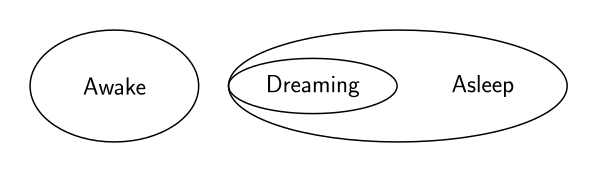
\includegraphics[width=1\textwidth,height=\textheight]{images/three-states.svg}
\caption[Relationship between wakefulness, dreaming and
sleep.]{Relationship between wakefulness, dreaming and
sleep.\footnotemark{}}\label{fig:three-states}
}
\end{figure}
\footnotetext{A simplified picture of the relationship between the
  states of wakefulness, sleep, and dreaming. Wakefulness and sleep are
  mutually exclusive. Dreaming only occurs in the sleep state.}

The phenomenon of \href{https://en.wikipedia.org/wiki/Lucid_dream}{lucid
dreaming} was scientifically established only in the 1980s.
Psychophysiological research has since discovered that it occurs in
\href{https://en.wikipedia.org/wiki/Rapid_eye_movement_sleep}{Rapid Eye
Movement (REM) sleep} and is as vivid---if not more vivid than---a
normal dream. Nevertheless, the subject who is dreaming is aware that he
or she is dreaming and, moreover, can volitionally alter the dream,
unlike the regular dreamer \protect\hyperlink{ref-laberge85}{{[}26{]}},
\protect\hyperlink{ref-laberge2000}{{[}27{]}}. This means that the lucid
dreamer occupies a paradoxical state at the borderline between sleep and
wakefulness in which the body is essentially in REM sleep, but the mind
is aware that it is dreaming, and is capable of controlling the dream.
Both the dream experience, and the fact that it was a conscious dream,
can be recalled during the wakeful state. After the recognition and
acceptance of lucid dreaming as a legitimate mental state, we may
represent the relationship between wakefulness, sleep, and dreaming by
the modified Venn diagram shown in \cref{fig:lucid}.

\begin{figure}
\hypertarget{fig:lucid}{%
\centering
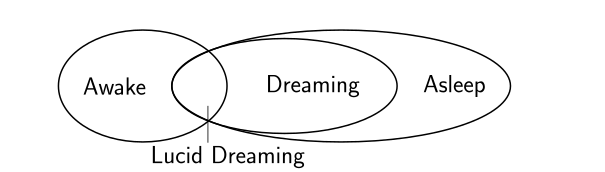
\includegraphics[width=1\textwidth,height=\textheight]{images/lucid.svg}
\caption[Modified relationship between wakefulness, dreaming and
sleep.]{Modified relationship between wakefulness, dreaming and
sleep.\footnotemark{}}\label{fig:lucid}
}
\end{figure}
\footnotetext{Modified, simplified relationship between wakefulness,
  dreaming, and sleep after the recognition and acceptance of lucid
  dreaming as a legitimate mental state. Lucid dreamers are mentally
  aware that they are dreaming and have conscious control over their
  dreams, while paradoxically, their bodies are asleep.}

It is tempting to conjecture that Tesla, working in his virtual
laboratory, functioned one level above the lucid dream, in being both
physically and mentally awake while inwardly running his mental
simulations with all the concentrated power, vividness, automaticity,
and verisimilitude of the dreaming mind.

\hypertarget{questions-vivid-visualization-and-virtual-laboratory}{%
\subsubsection{Questions: vivid visualization and virtual
laboratory}\label{questions-vivid-visualization-and-virtual-laboratory}}

Tesla's virtual laboratory is so unusual as to beggar belief. However,
Tesla was a scientist and engineer, schooled in accurate observation and
respect for objective truth. Moreover, his mode of working in his
virtual laboratory, without blueprints and prototypes, confounded and
frustrated his co-workers. So we may safely assume that Tesla indeed ran
his motor, examined its wear and tear, and then machined it to
compensate for that, all in his mind
\protect\hyperlink{ref-oneill80}{{[}2{]}} (p 58). This leads to many
tantalizing questions, including these:

\begin{enumerate}
\tightlist
\item
  Very simply, how did he do it?
\item
  What are the prerequisites for an imagination as vivid as Tesla's?
\item
  How does one achieve his intensity of visualization while wide awake?
\item
  What is the peculiar state in which Tesla's mind operated while he ran
  his virtual laboratory? Specifically, was Tesla's mind in a state of
  daydreaming, hallucination, lucid dreaming, visual thinking, or some
  as yet unknown mode, during his experiments?
\item
  Did Tesla simply visualize only the motion, or did he visualize the
  electricity too?
\item
  How does one visualize electricity?
\item
  Is precise scientific knowledge a pre-requisite for visualization as
  in the case of the virtual laboratory? In other words, does a person
  with such faculties need to know, in addition, the laws of physics and
  material properties in order to conduct experiments like Tesla?
\item
  Can the ordinary person acquire the skills needed for a virtual
  laboratory by suitable training and practice as is done in sport or
  dance?
\end{enumerate}

These fascinating questions are worthy of exploration, especially since
we are so familiar with
\href{https://en.wikipedia.org/wiki/Virtual_reality}{\emph{virtual
reality}} in computer games and simulations nowadays. Using this
language, it is clear that Tesla had replicated reality in his mind and
was running a virtual laboratory there.

\hypertarget{eccentricities-of-habit-and-behaviour}{%
\subsection{Eccentricities of habit and
behaviour}\label{eccentricities-of-habit-and-behaviour}}

Apart from his senses and vivid visualization, Tesla's body, habits,
will power, and social interactions all exhibited anomalies that merit
mention and reflection. Although he suffered a mental breakdown at 25,
and was prone to nervous exhaustion after long periods without rest, his
body exhibited remarkable features. Tesla had a superhuman appetite for
work. He was ``able to work thirty-eight years almost without a day's
interruption, and {[}could{]} find himself still strong and fresh in
body and mind'' \protect\hyperlink{ref-john83}{{[}1{]}}. He also had
enormous will power that could not only sustain a punishing schedule but
could also permanently banish undesirable habits that he had formed,
once he was so convinced. Some of his more notable traits are enumerated
below:

\begin{enumerate}
\tightlist
\item
  During his first year at the Polytechnic at Graz, he ``regularly
  started {[}his{]} work at three o'clock in the morning and continued
  until eleven at night, no Sundays or holidays excepted''
  \protect\hyperlink{ref-john83}{{[}1{]}}.
\item
  Tesla excelled at languages and knew English, French, German, Italian
  and the Slavic dialects \protect\hyperlink{ref-cheney81}{{[}3{]}} (p
  14).
\item
  He had a prodigious memory and could store entire logarithmic tables
  in his mind \protect\hyperlink{ref-cheney81}{{[}3{]}} (p 14).
\item
  He was left-handed but later became ambidextrous
  \protect\hyperlink{ref-oneill80}{{[}2{]}}.
\item
  He was not good at drawing \protect\hyperlink{ref-john83}{{[}1{]}}.
\item
  At the age of fifty-nine, when he slipped on icy ground, he righted
  himself like a cat while in the air and landed on his feet
  \protect\hyperlink{ref-john83}{{[}1{]}}.
\item
  At sixty-three his body shape and weight had remained unchanged for
  thirty-five years \protect\hyperlink{ref-john83}{{[}1{]}}.
\item
  He was attracted to gambling but gave it up when admonished by his
  parents. He not only ``conquered {[}his{]} passion then and there
  \ldots{} {[}but also{]} \ldots{} tore it from {[}his{]} heart so as
  not to leave even a trace of desire
  \protect\hyperlink{ref-john83}{{[}1{]}}.
\item
  He took up smoking, but on realizing that it would ruin his health,
  gave it up permanently \protect\hyperlink{ref-john83}{{[}1{]}}.
\item
  When Tesla discovered that the innocent cup of coffee he consumed
  every morning could precipitate heart trouble, he discontinued it by
  strenuous will \protect\hyperlink{ref-john83}{{[}1{]}}.
\end{enumerate}

He saw his conquest of bad habits in a different light from most people.
He said:

\begin{quote}
In this way I checked and bridled other habits and passions and have not
only preserved my life but derived an immense amount of satisfaction
from what most men would consider privation and sacrifice.
\protect\hyperlink{ref-john83}{{[}1{]}}
\end{quote}

One interesting question that arises is whether Tesla's extraordinary
visualization was in any way related to his tremendous will power.

\hypertarget{integrity-and-moral-sense}{%
\subsubsection{Integrity and moral
sense}\label{integrity-and-moral-sense}}

Tesla was a humanist who desired to use his mind for the freedom of all
mankind from the thralldom of matter. He wanted to liberate mankind from
drudgery using his magical inventions. While this idealistic vision
never left until the end, Tesla was singularly inept in his business
dealings. Indeed, one academic who teaches engineering management, and
is a lifelong Tesla enthusiast and biographer, has written that he uses
Tesla to teach his students how \emph{not} to run their business affairs
\protect\hyperlink{ref-lomas99}{{[}5{]}}. Two incidents that well
illustrate not only Tesla's integrity and moral sense but also his
business \href{https://www.thefreedictionary.com/naivete}{naïveté} are
noted below.

Thomas Edison once offered Tesla the then staggering sum of USD 50,000
for improving motor and generator designs. Tesla assiduously applied
himself to the changes and gave the Edison company several very
profitable patents in the process. When Tesla asked for the USD 50,000,
Edison is reported to have replied, ``Tesla, you don't understand our
American humor,'' and reneged on his promise
\protect\hyperlink{ref-tesla-wiki}{{[}6{]}}. Tesla promptly resigned.

The \href{https://en.wikipedia.org/wiki/War_of_the_currents}{``War of
the Currents''} \protect\hyperlink{ref-cheney81}{{[}3{]}} (chapter 5)
between DC and AC, waged between Thomas Edison and George Westinghouse,
left both almost bankrupt. Tesla, feeling loyalty and generosity toward
his new backer, Westinghouse, did not re-negotiate his patent royalties
but rather released Westinghouse altogether. In the process, he lost
what would have amounted to almost USD 12,000,000 in royalties
\protect\hyperlink{ref-cheney81}{{[}3{]}} (p 48--49). Tragically, toward
the end of his life, he was plagued by a chronic shortage of funds.

\hypertarget{tesla-as-a-humanist}{%
\subsubsection{Tesla as a humanist}\label{tesla-as-a-humanist}}

Tesla was unambiguous about the place of the inventor in society and of
his own role in life. The opening paragraph of his autobiography, which
may be called his
\href{https://en.wikipedia.org/wiki/Mission_statement}{\emph{mission
statement}}, begins thus:

\begin{quote}
The progressive development of man is vitally dependent on invention. It
is the most important product of his creative brain. Its ultimate
purpose is the complete mastery of mind over the material world, the
harnessing of the forces of nature to human needs. This is the difficult
task of the inventor who is often misunderstood and unrewarded. But he
finds ample compensation in the pleasing exercises of his powers and in
the knowledge of being one of that exceptionally privileged class
without whom the race would have long ago perished in the bitter
struggle against pitiless elements.
\protect\hyperlink{ref-john83}{{[}1{]}}
\end{quote}

Besides his innumerable inventions, he had also discovered the
following, each of which was later ``re-discovered'' by others who won
Nobel Prizes \protect\hyperlink{ref-oneill80}{{[}2{]}} (p 166):

\begin{enumerate}
\tightlist
\item
  \href{https://en.wikipedia.org/wiki/Cosmic_ray}{Cosmic rays};
\item
  Artificial
  \href{https://www.britannica.com/science/radioactivity}{radioactivity};
\item
  Disintegrating beam of electrified particles or
  \href{https://en.wikipedia.org/wiki/Particle_accelerator}{atom
  smasher};
\item
  \href{https://en.wikipedia.org/wiki/Electron_microscope}{Electron
  microscope}; and
\item
  Very special radiation or
  \href{https://en.wikipedia.org/wiki/X-ray}{X-rays}.
\end{enumerate}

Tesla was also the rightful inventor of radio, as established by the US
Patent and Trademark Office after his death, although
\href{https://en.wikipedia.org/wiki/Guglielmo_Marconi}{Guglielmo
Marconi} won the Nobel Prize for it
\protect\hyperlink{ref-tesla-home}{{[}7{]}}. It is regrettable that
Tesla was not only a man ahead of his time, but also one whom society
failed to recognize and reward, and whom time has literally forgotten.

\hypertarget{falling-asleep}{%
\subsubsection{Falling asleep}\label{falling-asleep}}

Tesla, being an experimental scientist, was an extremely keen observer.
The merit in studying his mind is that he brought his powers of
scientific observation to bear on his own mental processes and inner
experiences. We therefore have a window into the subjective mind of an
extraordinary person, impartially and accurately documented by himself.
Tesla fell asleep in a different way than most of us do, and he
described it thus:

\begin{quote}
When I close my eyes I invariably observe first, a background of very
dark and uniform blue, not unlike the sky on a clear but starless night.
In a few seconds this field becomes animated with innumerable
scintillating flakes of green, arranged in several layers and advancing
towards me. Then there appears, to the right, a beautiful pattern of two
systems of parallel and closely spaced lines, at right angles to one
another, in all sorts of colors with yellow-green and gold
predominating. Immediately thereafter the lines grow brighter and the
whole is thickly sprinkled with dots of twinkling light. This picture
moves slowly across the field of vision and in about ten seconds
vanishes to the left, leaving behind a ground of rather unpleasant and
inert grey which quickly gives way to a billowy sea of clouds, seemingly
trying to mould themselves in living shapes. It is curious that I cannot
project a form into this grey until the second phase is reached. Every
time, before falling asleep, images of persons or objects flit before my
view. When I see them I know that I am about to lose consciousness. If
they are absent and refuse to come it means a sleepless night.
\protect\hyperlink{ref-john83}{{[}1{]}}
\end{quote}

\hypertarget{idiosyncrasies}{%
\subsubsection{Idiosyncrasies}\label{idiosyncrasies}}

Undoubted genius that he was, Tesla also exhibited traits that most of
us would consider anomalous, if not downright abnormal. He had an
abnormal fear of germs \protect\hyperlink{ref-cheney81}{{[}3{]}} (p
263--264) causing him to wash his hands several (but always a multiple
of three) times. While dining, he needed eighteen clean linen napkins at
the dining table \protect\hyperlink{ref-cheney81}{{[}3{]}} (p 1). He was
also extremely fond of pigeons and used to nurse and feed any sick
pigeons he found \protect\hyperlink{ref-cheney81}{{[}3{]}}. In his early
life, Tesla developed a number of what he called ``strange likes,
dislikes and habits'' \protect\hyperlink{ref-john83}{{[}1{]}}. His own
account of them is as follows:

\begin{quote}
During that period I contracted many strange likes, dislikes and habits,
some of which I can trace to external impressions while others are
unaccountable. I had a violent aversion against the earrings of women
but other ornaments, as bracelets, pleased me more or less according to
design. The sight of a pearl would almost give me a fit but I was
fascinated with the glitter of crystals or objects with sharp edges and
plane surfaces. I would not touch the hair of other people except,
perhaps, at the point of a revolver. I would get a fever by looking at a
peach and if a piece of camphor was anywhere in the house it caused me
the keenest discomfort. Even now I am not insensible to some of these
upsetting impulses. When I drop little squares of paper in a dish filled
with liquid, I always sense a peculiar and awful taste in my mouth. I
counted the steps in my walks and calculated the cubical contents of
soup plates, coffee cups and pieces of food---otherwise my meal was
unenjoyable. All repeated acts or operations I performed had to be
divisible by three and if I missed I felt impelled to do it all over
again, even if it took hours. \protect\hyperlink{ref-john83}{{[}1{]}}
\end{quote}

The above quirks of mind and habit suggest that Tesla experienced the
following anomalies of mind:

\begin{enumerate}
\tightlist
\item
  \href{https://en.wikipedia.org/wiki/Obsessive\%E2\%80\%93compulsive_disorder}{obsessive-compulsive
  disorder};
\item
  \href{https://en.wikipedia.org/wiki/Synesthesia}{synaesthesia}; and
\item
  \href{https://en.wikipedia.org/wiki/High-functioning_autism}{high-functioning
  autism}.
\end{enumerate}

His fixation on the number three and having to wash his hands three
times, have eighteen napkins on the table during meals, walking around a
building thrice before entering it, etc., are all symptomatic of
obsessive-compulsive disorder
\protect\hyperlink{ref-tesla-wiki}{{[}6{]}}. So, too, his counting the
number of steps in his walks, and the cubic capacity of his soup plates
and items of food and drink. Tesla's compulsion with germs and
cleanliness may be traced back to periods in his life when he made a
trans-Atlantic voyage without his luggage, and when he spent a year
digging ditches in the United States to make ends meet. He vowed after
these experiences that he would never use a towel twice
\protect\hyperlink{ref-lomas99}{{[}5{]}} (pp 167--168). One is reminded
in this context of how a deeply-felt regret can lead to an obsession, as
in the case of Lady Macbeth who famously said, ``Here's the smell of the
blood still: all the perfumes of Arabia will not sweeten this little
hand,'' {[}Shakespeare, \emph{Macbeth}, act 5, scene, 1, lines 50--1{]}.

Synaesthesia is a condition in which stimulation of one sensory modality
gives rise to a response in another modality
\protect\hyperlink{ref-marks00}{{[}28{]}},
\protect\hyperlink{ref-cytowic96}{{[}29{]}}. A synaesthete may ``taste''
a shape for example. It is tempting to speculate that Tesla's awful
taste when dropping paper squares into a liquid may be symptomatic of
synaesthesia. It would also be interesting to explore whether his
hyper-acute senses and cross-modal sensory responses influenced each
other.

Tesla's abnormal sensitivity to sounds, his single-minded absorption in
what fascinated him, his solitary work habits, his inability to see
through the dishonesty of some of his work associates, etc., all suggest
that he might have been autistic. However, he had no difficulties with
language and, in fact knew Göthe's \emph{Faust} by heart, along with
several Serbian poems. This juxtaposition of some of the strengths found
in the autistic with few of their deficiencies, has prompted some to
suggest that Tesla probably suffered from high-functioning autism
\protect\hyperlink{ref-blume04}{{[}30{]}} or from
\href{https://en.wikipedia.org/wiki/Asperger_syndrome}{Asperger's
syndrome} \protect\hyperlink{ref-tesla-faq}{{[}31{]}}, which is a rare
condition in which the autistic child is intelligent, highly verbal, and
near normal \protect\hyperlink{ref-frith90}{{[}32{]}}. This would
explain both his extraordinary mental faculties and also a number of his
mental quirks. The existence of
\href{https://en.wikipedia.org/wiki/Savant_syndrome}{``autistic idiot
savants''} \protect\hyperlink{ref-frith90}{{[}32{]}} (pp 84--85),
\protect\hyperlink{ref-savant2009}{{[}33{]}} who function with
super-human excellence in some areas of human endeavour but who are
lacking severely in others, suggests that some compensatory
mechanism---a sort of zero sum for the total mental capacity---might
explain the co-existence of both their ``islets of abilities'' and
concomitant deficits.

\hypertarget{questions-idiosyncrasies}{%
\subsubsection{Questions:
idiosyncrasies}\label{questions-idiosyncrasies}}

Given that Tesla was unusual in many ways, and could have had what are
labelled today as
\href{https://en.wikipedia.org/wiki/Varieties_of_Anomalous_Experience}{``certain
varieties of anomalous experience''}, the following questions suggest
themselves:

\begin{enumerate}
\tightlist
\item
  Were his abnormalities like synaesthesia and obsessive-compulsive
  disorder the result of his mental precocity and extraordinary visual
  sense?
\item
  Are such conditions a ``compensatory'' accompaniment of genius?
\item
  Was Tesla indeed autistic?
\item
  Could it be that Tesla had both the left and right hemispheres of his
  brain functioning well above the capacity of normal human beings?
  (Recall that when the word for an object was spoken he ``saw'' the
  object referred to as if it were right in front of his eyes.)
\item
  Could this have led to some ``cross-wiring'' of his senses?
\item
  Could it also have led to the mélange of genius and eccentricity seen
  in him?
\end{enumerate}

\hypertarget{teslas-grandiose-claims}{%
\subsection{Tesla's grandiose claims}\label{teslas-grandiose-claims}}

Tesla's plans were always grand. Typical of the visionary, he saw the
fruition of his discoveries in his mind and spoke of them even before
they had been realized. When commercial or financial imperatives
obstructed their realization, he was often sidelined or ridiculed by the
scientific establishment. Yet, the very things he envisioned then are
realities in our present age of semiconductors, computers, and the
Internet. To appreciate just how prophetic his vision was, let us look
at just one example: his ``World-System''. In the vocabulary of Tesla's
day, this system would be capable of:

\begin{quote}
\begin{enumerate}
\tightlist
\item
  The inter-connection of the existing telegraph exchanges or offices
  all over the world;
\item
  The establishment of a secret and non-interferable government
  telegraph service;
\item
  The inter-connection of all the present telephone exchanges or offices
  on the Globe;
\item
  The universal distribution of general news, by telegraph or telephone,
  in connection with the Press;
\item
  The establishment of such a `World-System' of intelligence
  transmission for exclusive private use;
\item
  The inter-connection and operation of all stock tickers of the world;
\item
  The establishment of a `World-System' of musical distribution, etc.;
\item
  The universal registration of time by cheap clocks indicating the hour
  with astronomical precision and requiring no attention whatever;
\item
  The world transmission of typed or handwritten characters, letters,
  checks, etc.;
\item
  The establishment of a universal marine service enabling the
  navigators of all ships to steer perfectly without compass, to
  determine the exact location, hour and speed, to prevent collisions
  and disasters, etc.;
\item
  The inauguration of a system of world-printing on land and sea; and
\item
  The world reproduction of photographic pictures and all kinds of
  drawings or records. \protect\hyperlink{ref-john83}{{[}1{]}}
\end{enumerate}
\end{quote}

Grandiose claims they may have been in his time. Today, the world-mind
has enlarged beyond measure compared to the pre-transistor days in which
Tesla lived. It is to his great credit that in a world of condensers and
coils, he could visualize what electricity was capable of, in the
service of mankind.

In his later years, he formulated grand plans to use lightning to
generate artificial rain to turn deserts into gardens
\protect\hyperlink{ref-john83}{{[}1{]}}. Another of Tesla's pet projects
was the wireless transmission of free electrical energy from which all
mankind could benefit \protect\hyperlink{ref-tesla-energy}{{[}34{]}}.
This was in keeping with his mission statement. It was also consistent
with the fact the earth receives its sum total of energy from the sun in
precisely the same fashion. Yet, such grandiose projects and claims led
to the marginalization of Tesla as a force in science. Are his claims of
tapping an infinite energy source all around us worth re-investigation
in these times when global warming and the finitude of fossil fuels is
forcing a re-examination of all energy options?

\hypertarget{tesla-and-swami-vivekananda}{%
\subsubsection{Tesla and Swami
Vivekananda}\label{tesla-and-swami-vivekananda}}

Ideas about unlimited, free energy might have found resonance with Tesla
after his meeting with the famous Hindu monk,
\href{https://en.wikipedia.org/wiki/Swami_Vivekananda}{Swami
Vivekananda}, who visited the United States in the 1890s
\protect\hyperlink{ref-tesla-home}{{[}7{]}},
\protect\hyperlink{ref-grotz}{{[}35{]}},
\protect\hyperlink{ref-dobson}{{[}36{]}}. It is held that Tesla met the
Swami in 1895--6 and that he was receptive to the ideas expressed in the
Sanskrit language of Hindu cosmology about a universal energy, called
\emph{prāṇa}, and the vehicle for it, called \emph{ākāśa}, literally the
medium for radiance. The exposure to the idea that everything is
floating in a sea of universal \emph{prāṇa} must have taken hold in his
fertile imagination and given rise to claims about the possibility of
free energy from the capture of solar ``cosmic rays'' that could be used
to drive machines. His biographer O'Neill states that---in an
unpublished article entitled ``Man's Greatest Achievement''---Tesla
speaks of mankind in general, saying
\protect\hyperlink{ref-oneill80}{{[}2{]}} (p 270):

\begin{quote}
There manifests itself in the fully developed being, Man, a desire
mysterious, inscrutable and irresistible: to imitate nature, to create,
to work himself the wonders he perceives \ldots{} Long ago, he
recognized that all perceptible matter comes from a primary substance,
or tenuity beyond conception, filling all space, the Akasa or
luminiferous ether, which is acted upon by the life-giving Prana or
creative force, calling into existence, in never ending cycles, all
things and phenomena. The primary substance, thrown into infinitesimal
whirls of prodigious velocity, becomes gross matter; the force
subsiding, the motion ceases, and matter disappears, reverting to the
primary substance.

Can Man control this grandest, most awe-inspiring of all processes in
nature? Can he harness her inexhaustible energies to perform all their
functions to his bidding, more still to cause them to operate simply by
the force of his will?
\end{quote}

The fact that Tesla, who did not know Sanskrit, used the words prāṇa and
ākāśa, lends support to the claim that he did indeed meet Swami
Vivekananda. Tesla's expression ``tenuity beyond conception''
corresponds perfectly with the statement \emph{``ta ākāśe na vidyante''}
meaning ``(this) ākāśa is imperceptible''
\protect\hyperlink{ref-agra01}{{[}37{]}} (p 92), showing Tesla's ability
to grasp abstruse philosophical points. Indeed, he did expound on
philosophy, and was in that sense a well-rounded scholar
\protect\hyperlink{ref-tesla-cosmic}{{[}38{]}}.

Post-Einsteinian physics has not found a need for \emph{ākāśa} or the
luminiferous ether, but there is a need for \emph{something}, regardless
of label. Indeed, in a recent article on the ether, it has been observed
that ``Physicists appear to need an ether on which to load all the
properties of the physical world they cannot otherwise explain. Ether,
alias the vacuum, exists. Void is anything but nothing''
\protect\hyperlink{ref-heil03}{{[}39{]}}.

\hypertarget{teslas-pigeon}{%
\subsubsection{Tesla's pigeon}\label{teslas-pigeon}}

Although possessed of mental abilities that could almost be termed
psychic, Tesla did not give vent to the expression of his spiritual side
\protect\hyperlink{ref-oneill80}{{[}2{]}}. Indeed, when once approached
by a team of engineers to join a psychological society for investigating
psychic phenomena, Tesla almost threw them out
\protect\hyperlink{ref-john83}{{[}1{]}}.

With regard to his neglected spiritual side, Tesla's pigeon fixation
affords an interesting story \protect\hyperlink{ref-cheney81}{{[}3{]}}.
Tesla loved one particular female pigeon, almost as he would love a
human being. He recalled that one night, as he was lying on his bed in
the dark, this pigeon flew in through the open window, as if to deliver
a message. He looked at her and realized that she had come to tell him
she was dying. As he looked at her, Tesla said, ``there came a light
from her eyes---two powerful beams of light''. He reaffirmed, ``Yes, it
was a real light, a powerful, dazzling, blinding light, a light more
intense than I had ever produced by the most powerful lamps in my
laboratory'' \protect\hyperlink{ref-cheney81}{{[}3{]}} (p 229). When
that pigeon died, Tesla ``knew'' that his life's work was finished.

Although Tesla never publicly gave expression to his religious or
spiritual beliefs, this pigeon episode inevitably calls for comparison
with the Biblical account of the baptism of Jesus by John the Baptist:
``\ldots{} and he saw the Spirit of God descending like a dove, and
lighting upon him \ldots{}'' {[}Matthew\textasciitilde3:17{]}.

\hypertarget{buckes-hypothesis-on-human-mental-evolution}{%
\subsection{Bucke's hypothesis on human mental
evolution}\label{buckes-hypothesis-on-human-mental-evolution}}

The medical doctor, Richard Maurice Bucke\footnote{Formerly Medical
  Superintendent of the Asylum for the Insane at London, Ontario, Canada},
writing at the beginning of the twentieth century, advanced the radical
hypothesis that evolution also applied to the human mind
\protect\hyperlink{ref-bucke48}{{[}9{]}}. Although he used the word
``evolution'', Bucke did not imply any particular engine, like Darwinian
natural selection, for driving mental evolution, but rather asserted
blandly ``that growth, evolution, development, \ldots{} has \ldots{}
always gone on, is going on now, and \ldots{} will always go on''
\protect\hyperlink{ref-bucke48}{{[}9{]}} (p 61).

As a lead-in to his idea of mental evolution, Bucke proposed, among
other things, that man's sense of colour, sense of fragrance, and
musical sense had all developed over time to their present state.
Accordingly, he proposed that human colour vision was a recent
evolutionary development. He suggested that as sensory perception
evolved, the vocabulary of languages kept pace to deal with this
increasing sophistication. Tracking the gradual development of the words
for different colours in ancient languages and literature, he suggested
that the perception and recognition of colours kept pace with each other
according to the tree illustrated in \cref{fig:colour-tree}. Bucke
claimed that:

\begin{quote}
When a new faculty appears in a race it will be found, in the very
beginning, in one individual of that race; later it will be found in a
few individuals; after a further time in a larger percentage of the
members of that race; still later in half the members; and so on, until,
after thousands of generations, an individual who misses having the
faculty is regarded as a monstrosity.
\protect\hyperlink{ref-bucke48}{{[}9{]}} (p 52)
\end{quote}

\begin{figure}
\hypertarget{fig:colour-tree}{%
\centering
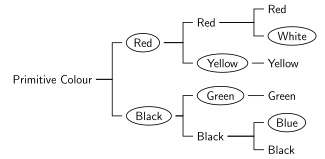
\includegraphics[width=1\textwidth,height=\textheight]{images/colour-perception-tree.svg}
\caption[Evolution of colour perception in human beings.]{Evolution of
colour perception in human
beings.\footnotemark{}}\label{fig:colour-tree}
}
\end{figure}
\footnotetext{Evolution of colour perception in human beings as
  conjectured by R M Bucke. This diagram is adapted from Bucke
  \protect\hyperlink{ref-bucke48}{{[}9{]}} (p 36). Time increases as one
  moves right. The circled colours were the ones newly recognized at any
  particular period. So, the progression of newly recognized colours was
  red/black, followed by yellow/green and later by white/blue. Bucke
  cites literary and scientific evidence in support of his conjecture.
  While his scientific arguments have now been supplanted, the literary
  arguments are still persuasive.}

Extrapolating from his suggested hypothetical development of colour
vision, etc., over time, Bucke postulated that the human mind also
evolved with time. He distinguished three progressive states of
consciousness so:

\begin{enumerate}
\item
  Simple consciousness that is possessed by the higher animals and man
  by which they are aware of their surroundings and also of their own
  bodies as integrated entities;
\item
  Self consciousness which is not present in animals, but only in man,
  whereby man becomes aware of himself as a distinct entity apart from
  the rest of the universe, and which allows him to treat his own mental
  states as objects of consciousness, and also allows communication by
  language; and
\item
  Cosmic consciousness which includes simple and self consciousness, but
  which in addition allows ``a consciousness of the cosmos, that is, of
  the life and order of the universe''
  \protect\hyperlink{ref-bucke48}{{[}9{]}} (p 3) and ``an intellectual
  enlightenment or illumination which alone would place the individual
  on a new plane of existence---would make him almost a member of a new
  species'' \protect\hyperlink{ref-bucke48}{{[}9{]}} (p 3). Bucke stated
  that the burden of his book was to expound the nature of this exalted
  state and identify some of its exemplars.
\end{enumerate}

While there have been many extraordinary spiritual leaders of humankind
with superior mental attributes, Tesla's phenomenal mental abilities
present one of the most prominent examples of such abilities in a man or
woman of science. Whether or not Tesla possessed ``cosmic
consciousness'' in accordance with Bucke's definition, we may
justifiably ask whether Tesla possessed a more evolved mind than the
ordinary human being. \emph{Or more precisely, was Tesla a
representative from our future, in which those possessing his faculties
would be more numerous than today?} It is a tantalizing question that
may have no clear cut answers for now.

\hypertarget{conclusions}{%
\subsection{Conclusions}\label{conclusions}}

Like \href{https://en.wikipedia.org/wiki/Icarus}{Icarus}, Tesla sought
the freedom of flight. Like
\href{https://en.wikipedia.org/wiki/Prometheus}{Prometheus}, Tesla
wrested the subtle fire of electricity from the realm of the invisible
and brought it down into the world of mortals. Like
\href{https://en.wikipedia.org/wiki/Zeus}{Zeus}, he wielded the
thunderbolt by creating lightning artificially. Like
\href{https://en.wikipedia.org/wiki/Archimedes}{Archimedes}, his
thoughts were always on a grand scale and he was not only the
theoretical mathematical physicist but also the practical
engineer-inventor.

Tesla was larger than life and greater than most of his fellow human
beings. He excelled in his intellect, power of will and visualization,
and his moral sense. He was unambiguous in his personal mission
statement about the social responsibility of the inventor-scientist as
one who ameliorates the life of his fellow human beings. He held that
the pleasure of discovery and invention was its own reward. He embraced
the insights that came to him through non-rational processes of thought.
Perhaps, he exercised, more symmetrically and to a greater degree than
most people, both the right and left hemispheres of his brain.

One rather sad, recurring theme in the biographies of Tesla is that he
was somehow a misfit either in the society in which he lived and worked,
or the times in which his life was enacted. Margaret Cheney's biography,
\emph{Tesla: Man Out of Time}, clearly shows this in its very title. As
does also the subtitle of Lomas's book
\protect\hyperlink{ref-lomas99}{{[}5{]}}, \emph{Nikola Tesla, Forgotten
Genius of Electricity}. Do these titles hold the key to Tesla's mystery?
\emph{Was Tesla from our future?}

The most important contribution of Tesla may not be the alternating
current grid, or the induction motor, or any of his other electrical
inventions. It may simply be the fact that he was a very unusual human
being with remarkable mental powers that most of us can only call
incredible or legendary. How did he come by them? Were his abilities the
result of some form of compensation, as in the autistic idiot savant,
\emph{or was it simply that Tesla was a man from our future who had torn
the veil of time to visit us and give us a glimpse of the future
capabilities of humankind?}

\hypertarget{acknowledgements}{%
\subsection{Acknowledgements}\label{acknowledgements}}

For helpful comments and discussions, I thank N Chandrasekhar, R
Gopalkrishnan, M Jegasothy, P Jones, M R Jupp, B Raguram, B Readhead,
and R Sivasankar.

\hypertarget{feedback}{%
\subsection{Feedback}\label{feedback}}

Please \href{mailto:feedback.swanlotus@gmail.com}{email me} your
comments and corrections.

\noindent A PDF version of this article is
\href{./mind-of-tesla.pdf}{available for download here}:

\begin{normalsize}

\begin{ttfamily}

\url{https://swanlotus.netlify.app/blogs/mind-of-tesla.pdf}

\end{ttfamily}

\end{normalsize}

\hypertarget{bibliography}{%
\section*{References}\label{bibliography}}
\addcontentsline{toc}{section}{References}

\hypertarget{refs}{}
\begin{CSLReferences}{0}{0}
\leavevmode\vadjust pre{\hypertarget{ref-john83}{}}%
\CSLLeftMargin{{[}1{]} }
\CSLRightInline{N. Tesla, {`{My Inventions: The Autobiography of Nikola
Tesla}'}, B. Johnston, Ed. Williston, VT, USA: Hart Brothers, 1983
{[}Online{]}. Available:
\url{http://www.tfcbooks.com/special/mi_link.htm}. {[}Accessed:
06-Jun-2002{]}}

\leavevmode\vadjust pre{\hypertarget{ref-oneill80}{}}%
\CSLLeftMargin{{[}2{]} }
\CSLRightInline{J. J. O' Neill, \emph{{Prodigal Genius: The Life of
Nikola Tesla}}. St Albans, Herts, UK: Granada Publishing, 1980. }

\leavevmode\vadjust pre{\hypertarget{ref-cheney81}{}}%
\CSLLeftMargin{{[}3{]} }
\CSLRightInline{M. Cheney, \emph{{Tesla: Man Out of Time}}. Englewood
Cliffs, NJ, USA: Prentice-Hall, 1981. }

\leavevmode\vadjust pre{\hypertarget{ref-seifer98}{}}%
\CSLLeftMargin{{[}4{]} }
\CSLRightInline{M. J. Seifer, \emph{{Wizard: The Life and Times of
Nikola Tesla : Biography of a Genius}}, Reprint. New York, NY, USA:
Citadel Press, 1998. }

\leavevmode\vadjust pre{\hypertarget{ref-lomas99}{}}%
\CSLLeftMargin{{[}5{]} }
\CSLRightInline{R. Lomas, \emph{{The Man Who Invented the Twentieth
Century: Nikola Tesla, Forgotten Genius of Electricity}}. London, UK:
Headline Book Publishing, 1999. }

\leavevmode\vadjust pre{\hypertarget{ref-tesla-wiki}{}}%
\CSLLeftMargin{{[}6{]} }
\CSLRightInline{---, {`{N}ikola {T}esla --- {Wikipedia}{,} the {F}ree
{E}ncyclopedia'}, 2021. {[}Online{]}. Available:
\url{https://en.wikipedia.org/wiki/Nikola_Tesla}. {[}Accessed:
23-Feb-2021{]}}

\leavevmode\vadjust pre{\hypertarget{ref-tesla-home}{}}%
\CSLLeftMargin{{[}7{]} }
\CSLRightInline{J. M. Newlight, {`{Nikola Tesla}'}. {[}Online{]}.
Available: \url{http://www.teslaplay.com/index.html}. {[}Accessed:
23-Feb-2021{]}}

\leavevmode\vadjust pre{\hypertarget{ref-tesla-pbs-bio}{}}%
\CSLLeftMargin{{[}8{]} }
\CSLRightInline{R. Uth and M. Cheney, {`{PBS: Tesla---Master of
Lightning: Who Was Nikola Tesla?}'}, 2004. {[}Online{]}. Available:
\url{https://www.pbs.org/tesla/}. {[}Accessed: 26-Jun-2006{]}}

\leavevmode\vadjust pre{\hypertarget{ref-bucke48}{}}%
\CSLLeftMargin{{[}9{]} }
\CSLRightInline{R. M. Bucke, \emph{{Cosmic Consciousness: A Study in the
Evolution of the Human Mind}}, 14th ed. New York, USA: E P Dutton, 1948.
}

\leavevmode\vadjust pre{\hypertarget{ref-tesla-personal}{}}%
\CSLLeftMargin{{[}10{]} }
\CSLRightInline{N. Tesla, {`{Some Personal Recollections}'},
\emph{Scientific American}, 1915 {[}Online{]}. Available:
\url{https://www.pbs.org/tesla/res/res_art01.html}. {[}Accessed:
06-Jun-2006{]}}

\leavevmode\vadjust pre{\hypertarget{ref-weisberg86}{}}%
\CSLLeftMargin{{[}11{]} }
\CSLRightInline{R. Weisberg, \emph{{Creativity: genius and other
myths}}. New York, NY, USA: W H Freeman, 1986. }

\leavevmode\vadjust pre{\hypertarget{ref-findlay37}{}}%
\CSLLeftMargin{{[}12{]} }
\CSLRightInline{A. Findlay, \emph{{A Hundred Years of Chemistry}}.
London, UK: Duckworth, 1937. }

\leavevmode\vadjust pre{\hypertarget{ref-kekules-dream}{}}%
\CSLLeftMargin{{[}13{]} }
\CSLRightInline{---, {`{Kekule's Dream}'}. {[}Online{]}. Available:
\url{https://www.youtube.com/watch?v=2NRwd-JJFm4}. {[}Accessed:
21-Feb-2021{]}}

\leavevmode\vadjust pre{\hypertarget{ref-justin06}{}}%
\CSLLeftMargin{{[}14{]} }
\CSLRightInline{R. G. Justin, {`{Otto Loewi's Great Dreams}'}, \emph{The
Permanente Journal}, vol. 10, no. 2, pp. 70--71, 2006 {[}Online{]}.
Available:
\url{http://www.thepermanentejournal.org/files/Summer2006/otto.pdf}.
{[}Accessed: 23-Feb-2021{]}}

\leavevmode\vadjust pre{\hypertarget{ref-loewi2014}{}}%
\CSLLeftMargin{{[}15{]} }
\CSLRightInline{A. N. McCoy and Y. S. Tan, {`{Otto Loewi (1873--1961):
Dreamer and Nobel laureate}'}, \emph{Singapore Medical Journal}, vol.
55, no. 1, pp. 3--4, 2014 {[}Online{]}. Available:
\url{https://www.ncbi.nlm.nih.gov/pmc/articles/PMC4291908/}.
{[}Accessed: 21-Feb-2021{]}}

\leavevmode\vadjust pre{\hypertarget{ref-springer89}{}}%
\CSLLeftMargin{{[}16{]} }
\CSLRightInline{S. P. Springer and G. Deutsch, Eds., \emph{{Left Brain,
Right Brain}}. New York, NY, USA: W H Freeman, 1989. }

\leavevmode\vadjust pre{\hypertarget{ref-silver02}{}}%
\CSLLeftMargin{{[}17{]} }
\CSLRightInline{L. K. Silverman, \emph{{Upside-Down Brilliance: The
Visual-Spatial Learner}}. Denver, CO, USA: De Leon Publishing, 2002. }

\leavevmode\vadjust pre{\hypertarget{ref-west91}{}}%
\CSLLeftMargin{{[}18{]} }
\CSLRightInline{T. G. West, \emph{{In the mind's eye: visual thinkers,
gifted people with learning difficulties, computer images, and the
ironies of creativity}}. Buffalo, NY, USA: Prometheus Books, 1991. }

\leavevmode\vadjust pre{\hypertarget{ref-koestler64}{}}%
\CSLLeftMargin{{[}19{]} }
\CSLRightInline{A. Koestler, \emph{{The Act of Creation}}. New York, NY,
USA: Macmillan, 1964. }

\leavevmode\vadjust pre{\hypertarget{ref-kanigel91}{}}%
\CSLLeftMargin{{[}20{]} }
\CSLRightInline{R. Kanigel, \emph{{The Man Who Knew Infinity: A Life of
the Genius Ramanujan}}. New York, NY, USA: Charles Scribner's Sons,
1991. }

\leavevmode\vadjust pre{\hypertarget{ref-mckim72}{}}%
\CSLLeftMargin{{[}21{]} }
\CSLRightInline{R. H. McKim, \emph{{Experiences in Visual Thinking}}.
Belmont, CA, USA: Brooks/Cole, 1972. }

\leavevmode\vadjust pre{\hypertarget{ref-hubel88}{}}%
\CSLLeftMargin{{[}22{]} }
\CSLRightInline{D. H. Hubel, \emph{{Eye, Brain, and Vision}}. New York,
NY, USA: Scientific American Library, 1988. }

\leavevmode\vadjust pre{\hypertarget{ref-zeki93}{}}%
\CSLLeftMargin{{[}23{]} }
\CSLRightInline{S. Zeki, \emph{{A Vision of the Brain}}. Oxford, UK:
Blackwell Scientific Publications, 1993. }

\leavevmode\vadjust pre{\hypertarget{ref-pvi97}{}}%
\CSLLeftMargin{{[}24{]} }
\CSLRightInline{W. R. Hendee and P. N. T. Wells, Eds., \emph{{The
Perception of Visual Information}}, 2nd ed. New York, USA: Springer
Verlag, 1997. }

\leavevmode\vadjust pre{\hypertarget{ref-einstein-quote}{}}%
\CSLLeftMargin{{[}25{]} }
\CSLRightInline{A. Einstein, {`{Quote by Albert Einstein: {``I am enough
of an artist to draw freely upon my \ldots{}''}}'}, 2021. {[}Online{]}.
Available:
\url{https://www.goodreads.com/quotes/2177-i-am-enough-of-an-artist-to-draw-freely-upon}.
{[}Accessed: 24-Feb-2021{]}}

\leavevmode\vadjust pre{\hypertarget{ref-laberge85}{}}%
\CSLLeftMargin{{[}26{]} }
\CSLRightInline{S. LaBerge, \emph{{Lucid Dreaming}}. Los Angeles, CA,
USA: Jeremy P Tarcher, 1985. }

\leavevmode\vadjust pre{\hypertarget{ref-laberge2000}{}}%
\CSLLeftMargin{{[}27{]} }
\CSLRightInline{S. LaBerge and J. Gackenbach, {`{Lucid Dreaming}'}, in
\emph{{Varieties of Anomalous Experience: Examining the Scientific
Evidence}}, E. Cardeña, S. J. Lynn, and S. Krippner, Eds. Washington,
DC, USA: American Psychological Association, 2000, pp. 151--182. }

\leavevmode\vadjust pre{\hypertarget{ref-marks00}{}}%
\CSLLeftMargin{{[}28{]} }
\CSLRightInline{L. E. Marks, {`Synesthesia'}, in \emph{{Varieties of
Anomalous Experience: Examining the Scientific Evidence}}, E. Cardeña,
S. J. Lynn, and S. Krippner, Eds. Washington, DC, USA: American
Psychological Association, 2000, pp. 121--149. }

\leavevmode\vadjust pre{\hypertarget{ref-cytowic96}{}}%
\CSLLeftMargin{{[}29{]} }
\CSLRightInline{R. E. Cytowic, \emph{{The Man Who Tasted Shapes}}.
London, UK: Abacus, 1996. }

\leavevmode\vadjust pre{\hypertarget{ref-blume04}{}}%
\CSLLeftMargin{{[}30{]} }
\CSLRightInline{H. Blume, {`{Autism \& The Internet or It's The Wiring,
Stupid}'}, 1997. {[}Online{]}. Available:
\url{http://web.mit.edu/comm-forum/legacy/papers/blume.html}.
{[}Accessed: 23-Feb-2021{]}}

\leavevmode\vadjust pre{\hypertarget{ref-tesla-faq}{}}%
\CSLLeftMargin{{[}31{]} }
\CSLRightInline{G. Peterson, {`{Tesla's Mind \textbar{} Tesla FAQ No. 4
\textbar{} Interesting Facts About Nikola Tesla}'}. {[}Online{]}.
Available: \url{http://www.tfcbooks.com/teslafaq/q\&a_004.htm}.
{[}Accessed: 26-Jun-2006{]}}

\leavevmode\vadjust pre{\hypertarget{ref-frith90}{}}%
\CSLLeftMargin{{[}32{]} }
\CSLRightInline{U. Frith, \emph{{Autism: Explaining the Enigma}}.
Oxford, UK: Basil Blackwell, 1990. }

\leavevmode\vadjust pre{\hypertarget{ref-savant2009}{}}%
\CSLLeftMargin{{[}33{]} }
\CSLRightInline{D. A. Treffert, {`The savant syndrome: An extraordinary
condition. A synopsis: Past, present, future'}, \emph{Philosophical
Transactions of the Royal Society of London. Series B, Biological
sciences}, vol. 364, no. 1522, pp. 1351--1357 {[}Online{]}. Available:
\url{https://www.ncbi.nlm.nih.gov/pmc/articles/PMC2677584/}.
{[}Accessed: 22-Feb-2021{]}}

\leavevmode\vadjust pre{\hypertarget{ref-tesla-energy}{}}%
\CSLLeftMargin{{[}34{]} }
\CSLRightInline{N. Tesla, {`{The Problem Of Increasing Human Energy:
With Special References to the Harnessing of the Sun's Energy}'}.
{[}Online{]}. Available:
\url{https://www.pbs.org/tesla/res/res_art09.html}. {[}Accessed:
26-Jun-2006{]}}

\leavevmode\vadjust pre{\hypertarget{ref-grotz}{}}%
\CSLLeftMargin{{[}35{]} }
\CSLRightInline{T. Grotz, {`{The Influence of Vedic Philosophy on Nikola
Tesla's Understanding of Free Energy}'}, 1997. {[}Online{]}. Available:
\url{http://mountainman.com.au/aether_1.html}. {[}Accessed:
06-Jun-2006{]}}

\leavevmode\vadjust pre{\hypertarget{ref-dobson}{}}%
\CSLLeftMargin{{[}36{]} }
\CSLRightInline{J. Dobson, {`{The Equations of Maya}'}, 1993.
{[}Online{]}. Available:
\url{http://quanta-gaia.org/dobson/EquationsOfMaya.html}. {[}Accessed:
23-Feb-2021{]}}

\leavevmode\vadjust pre{\hypertarget{ref-agra01}{}}%
\CSLLeftMargin{{[}37{]} }
\CSLRightInline{Madan Mohan Agrawal, Ed., \emph{{Six Systems of Indian
Philosophy}}. New Delhi, India: Chaukamba Sanskrit Pratishthan, 2001. }

\leavevmode\vadjust pre{\hypertarget{ref-tesla-cosmic}{}}%
\CSLLeftMargin{{[}38{]} }
\CSLRightInline{N. Tesla, {`{How Cosmic Forces Shape Our Destinies:
({``Did the War Cause the Italian Earthquake''})}'}. {[}Online{]}.
Available: \url{https://www.pbs.org/tesla/res/res_art10.html}.
{[}Accessed: 26-Jun-2006{]}}

\leavevmode\vadjust pre{\hypertarget{ref-heil03}{}}%
\CSLLeftMargin{{[}39{]} }
\CSLRightInline{J. L. Heilbron, {`Ether'}, in \emph{{The Oxford
Companion to the History of Modern Science}}, J. L. Heilbron, Ed. Oxford
University Press, 2003. }

\end{CSLReferences}



\end{document}
